% (c) 2014 Daniele Masini - d.masini.it@gmail.com
\chapter{Successioni e progressioni numeriche}

\section{Successioni numeriche}

Intuitivamente per successione si intende una sequenza ordinata di infiniti elementi. Ci sarà quindi il primo elemento, il secondo, il terzo e così via.
Gli elementi che costituiscono una successione vengono anche detti \emph{termini} della successione.
Nel nostro caso siamo interessati alle successioni che hanno come termini i numeri e per questo si studieranno le successioni numeriche.

Sono esempi di successioni numeriche:

\begin{itemize}
\item i numeri pari: 2, 4, 6, 8, 10, 12, \ldots
\item i numeri dispari: 1, 3, 5, 7, 9, 11, 13, \ldots
\item i numeri quadrati perfetti: 1, 4, 9, 16, 25, \ldots
\item i reciproci dei numeri naturali: 1, $\dfrac{1}{2}$, $\dfrac{1}{3}$, $\dfrac{1}{4}$, $\dfrac{1}{5}$, \ldots
\end{itemize}

Formalmente si può dare la seguente definizione

\begin{definizione}
Si definisce \emph{successione numerica} un'applicazione $f$ dall'insieme $\insN_0$ in un'inseme $A$, cioè $f:\insN_0\to A$, che associa ad ogni $n\in\insN_0$ un elemento $a_n\in A$, ovvero $a_n = f(n)$.
\end{definizione}

Quindi una successione è costituita da una sequenza di termini
\[a_1\text{, }a_2\text{, }a_3\text{, }\ldots\text{, }a_n\text{, }\ldots\]
che, in genere, si rappresenta scrivendo semplicemente $\{a_n\}$.

Per i nostri scopi, l'insieme $A$ coincide con $\insR$.

Sebbene sia composta da un'infinità numerabile di termini ordinati, una successione non può essere assimilata ad un insieme numerabile, poiché a differenza di questi ultimi, in una successione numerica l'ordine nel quale si trovano i termini è rilevante e lo stesso termine può anche comparire più volte.

Per definire una successione, il metodo più utilizzato è quello di utilizzare una formula chiusa che specifica la relazione tra il generico numero $n\in\insN_0$ e il relativo termine della successione $a_n$. Per esempio, la successione dei numeri pari può essere definita specificando come viene ``calcolato'' il suo generico termine, cioè $a_n=2n$. In maniera analoga possiamo definire la successione armonica, quella dei reciproci dei numeri naturali, indicando la formula che rappresenta il suo termine $n$-esimo $a_n=\frac{1}{n}$.

\pagebreak
\begin{exrig}
\begin{esempio}
Definire la successione dei quadrati perfetti.

Per quadrato perfetto si intende il quadrato di un numero naturale, quindi bisogna trovare la formula che per ogni numero $n\in\insN$ ci fornisca il suo quadrato. Tale formula è $n^2$. Si può pertanto scrivere la successione come:
\[\{a_n\}\text{~~con~~}a_n=n^2\qquad\text{o più semplicemente}\qquad\left\{n^2\right\}.\]
\end{esempio}

\begin{esempio}\label{es:def_ricorsiva}
Definire la successione dei numeri dispari.

I numeri dispari sono 1, 3, 5, 7, \ldots{} ovvero per $n=1$ si ha $a_1=1$, per $n=2$ si ha $a_2=3$, per $n=3$ si ha $a_3=5$, \ldots{} Quindi, per ogni $n$ considerato $a_n$ è sempre un'unità meno del doppio di $n$, ovvero $2n-1$. Quindi la successione può essere scritta come
\[\{a_n\}\text{~~con~~}a_n=2n-1\qquad\text{o più semplicemente}\qquad\{2n-1\}.\]

Per definire tale successione si può anche far leva su un'altra caratteristica: dalla sequenza dei numeri dispari è evidente che ogni numero dispari è pari al precedente più 2. Quindi si può stabilire il valore del primo elemento $a_1=1$ e indicare che ogni elemento si ricava da quello precedente aggiungendovi 2, cioè utilizzando la scrittura seguente:
\[\{a_n\}=\left\{\begin{array}{l}a_1=1\\a_{n+1}=a_n+2\end{array}\right..\]
\end{esempio}
\end{exrig}

Come abbiamo visto nell'esempio~\ref{es:def_ricorsiva}, le successioni possono anche essere definite ricorsivamente, cioè indicando il valore dei primi termini e quindi fornendo una relazione che lega il termine generico agli altri.
Quest'ultimo tipo di definizione è utilizzato, ad esempio, nel caso della successione di Fibonacci\footnote{la successione è nata dal problema di definire il numero totale di conigli generati a distanza di un anno a partire da una coppia e sapendo che ogni coppia mette al mondo una coppia di conigli al mese. Tale successione ha interessanti riscontri anche in altri ambiti.}
\[\{a_n\}=\left\{\begin{array}{l}a_1=1\\a_2=1\\a_{n+2}=a_{n+1}+a_{n}\end{array}\right.\]
in questo modo, si indica il valore dei primi due termini $a_1$ e $a_2$ e si stabilisce che il generico termine è dato dalla somma dei suoi due precedenti. La successione assume pertanto i valori: 1, 1, 2, 3, 5, 8, 13, 21, 34, \ldots

Ovviamente, non è detto che le successioni siano definite per qualunque $n\in\insN_0$ ma, in maniera del tutto analoga a quanto visto per le funzioni, ogni successione avrà il proprio dominio $\Dom \subseteq \insN_0$ ed un proprio insieme immagine (o sostegno) $\IM \subseteq A$.

\begin{exrig}
\begin{esempio}
Determinare il dominio della successione $\left\{\dfrac{2n^2}{n-1}\right\}$.

La successione data, ovvero la relativa funzione $f:\insN_0 \to \insR$, $f(n) = \dfrac{2n^2}{n-1}$ è definita $\forall n\in\insN_0-\{1\}$ poiché per $n=1$ il denominatore si annulla e l'espressione perde di significato. Quindi il suo dominio è $\Dom = \insN_0-\{1\}$.
\end{esempio}
\begin{esempio}
Determinare il dominio della successione $\left\{\dfrac{n-5}{n^2-4}\right\}$.

Ricordando i prodotti notevoli, l'espressione $\dfrac{n-5}{n^2-4}$ può essere scritta come
\[\dfrac{n-5}{n^2-4} = \dfrac{n-5}{(n+2)(n-2)}\]
quindi la frazione esiste per qualunque $n\in\insN_0-\{2\}$, che coincide con il dominio $\Dom$ della successione data.
\end{esempio}

\begin{esempio}
Determinare il dominio della successione $\left\{\dfrac{n^2+4}{n-\sqrt{3}}\right\}$.

L'espressione $\dfrac{n^2+4}{n-\sqrt{3}}$ esiste per qualunque $n \neq \sqrt{3}$, ma poiché $\sqrt{3}\notin\insN$, l'espressione esiste $\forall n\in\insN_0$. In tal caso $\Dom = \insN_0$.
\end{esempio}
\end{exrig}

Come avviene per le altre funzioni, anche le successioni possono essere rappresentate nel piano cartesiano, dove sull'asse delle ascisse vengono riportati i valori di $n\in\insN_0$ e su quello delle ordinate i valori assunti dal relativo termine della successione $a_n$, quindi il generico punto $P_n$ avrà coordinate $(n;a_n)$. Si ottiene così una serie di punti isolati che delinea l'andamento della successione stessa. Ad esempio, considerando la successione armonica si ha $a_1 = 1$, $a_2=\frac{1}{2}$, $a_3=\frac{1}{3}$, $a_4=\frac{1}{4}$, $a_5=\frac{1}{5}$, \ldots, pertanto i punti del suo grafico saranno: $P_1(1;1)$, $P_2\left(2;\frac{1}{2}\right)$, $P_3\left(3;\frac{1}{3}\right)$, $P_4\left(4;\frac{1}{4}\right)$, $P_5\left(5;\frac{1}{5}\right)$, \ldots{} (figura~\ref{fig:8a.1}).

\begin{figure}[hbt]
 \begin{minipage}[t]{\textwidth}
\centering
 % (c) 2014 Daniele Masini - d.masini.it@gmail.com
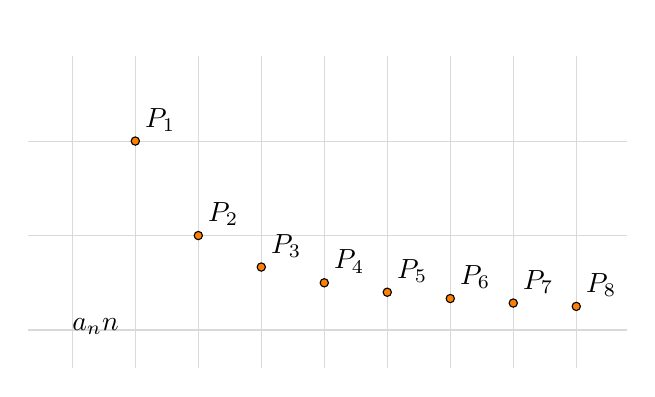
\begin{tikzpicture}[x=8mm, y=24mm]
%[step=8mm]
\draw[xstep=1,ystep=.5,color=gray!30] (-.7,-.2) grid (8.8,1.45);
\tkzInit[xmin=-.7,xmax=8,ymin=-.2,ymax=0.9]
\clip (-.7,-.2) rectangle (8.8,1.6);
\begin{scope}[font=\small]
  \tkzLabelY[orig=false,label options={left=1pt}]
  \tkzDrawY[label=$a_n$]
  \tkzLabelX[orig=false,label options={below=1pt}]
  \tkzDrawX[label=$n$]
%  \node[below left] at (0,0) {$O$};
\end{scope}
\foreach \x in {1,...,8}
{
  \draw[fill=orange] (\x,1/\x) circle (1.5pt);
  \node[above right] at (\x,1/\x) {$P_{\x}$};
}
\end{tikzpicture}

\caption{Grafico di $\left\{\frac{1}{n}\right\}$.}\label{fig:8a.1}
 \end{minipage}\hfil
\end{figure}

\begin{exrig}
\begin{esempio}
Rappresentare nel piano cartesiano la successione $\left\{\dfrac{n^2-1}{n+2}\right\}$.

Calcoliamo i primi 6 termini della successione e riportiamoli in una tabella
\begin{center}
\begin{tabular} {*{7}{c}}
\toprule
$n$ & 1 & 2 & 3 & 4 & 5 & 6\\
$\dfrac{n^2-1}{n+2}$ & 0 & $\dfrac{3}{4}$ & $\dfrac{8}{5}$ & $\dfrac{15}{6}$ & $\dfrac{24}{7}$ & $\dfrac{35}{8}$\\
\bottomrule
\end{tabular}
\end{center}
I punti da rappresentare nel piano cartesiano saranno quindi $P_1(1;0)$, $P_2\left(2;\frac{3}{4}\right)$, $P_3\left(3;\frac{8}{5}\right)$, $P_4\left(4;\frac{15}{6}\right)$, $P_5\left(5;\frac{24}{7}\right)$, $P_6\left(6;\frac{35}{8}\right)$.
\begin{center}
 % (c) 2014 Daniele Masini - d.masini.it@gmail.com
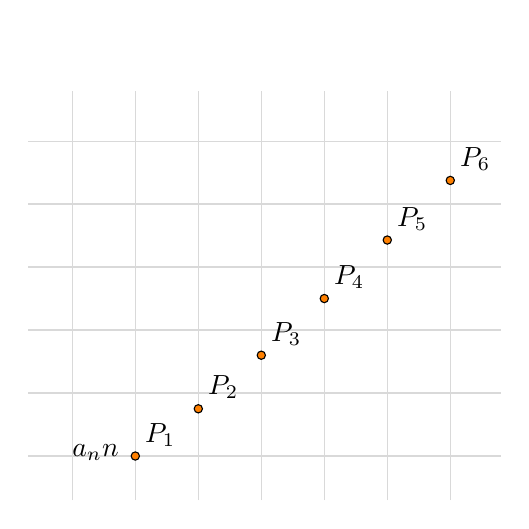
\begin{tikzpicture}[x=8mm, y=8mm]
\draw[step=8mm,color=gray!30] (-.7,-.7) grid (6.8,5.8);
\tkzInit[xmin=-0.7,xmax=6,ymin=-0.7,ymax=5]
\clip (-.7,-.7) rectangle (6.8,6.8);
\begin{scope}[font=\small]
  \tkzLabelY[orig=false,label options={left=1pt}]
  \tkzDrawY[label=$a_n$]
  \tkzLabelX[orig=false,label options={below=1pt}]
  \tkzDrawX[label=$n$]
%  \node[below left] at (0,0) {$O$};
\end{scope}
\foreach \x in {1,...,6}
{
  \draw[fill=orange] (\x,{\x*\x-1)/(\x+2)}) circle (1.5pt);
  \node[above right] at (\x,{\x*\x-1)/(\x+2)}) {$P_{\x}$};
}
\end{tikzpicture}

\end{center}
\end{esempio}

\begin{esempio}
Rappresentare nel piano cartesiano la successione $\left\{\dfrac{n}{n^2+1}\right\}$.

Lasciamo al lettore l'esercizio
\begin{center}
\begin{tabular} {*{7}{c}}
\toprule
$n$ & 1 & 2 & 3 & 4 & 5 & 6\\
$\dfrac{n}{n^2+1}$ & \ldots & \ldots & \ldots & \ldots & \ldots & \ldots\\
\bottomrule
\end{tabular}
\end{center}

\begin{center}
 % (c) 2014 Daniele Masini - d.masini.it@gmail.com
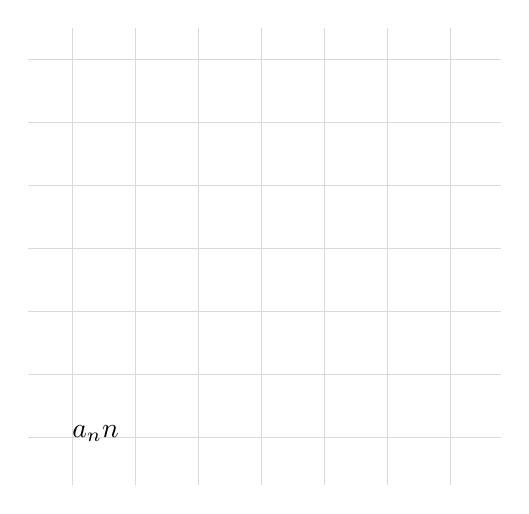
\begin{tikzpicture}[x=8mm, y=40mm]
\draw[step=8mm,color=gray!30] (-.7,-.15) grid (6.8,1.3);
\tkzInit[xmin=-.7,xmax=6,ymin=-.15,ymax=0.7]
\clip (-.7,-.15) rectangle (6.8,1.3);
\begin{scope}[font=\small]
  \tkzLabelY[orig=false,label options={left=1pt}]
  \tkzDrawY[label=$a_n$]
  \tkzLabelX[orig=false,label options={below=1pt}]
  \tkzDrawX[label=$n$]
%  \node[below left] at (0,0) {$O$};
\end{scope}
\end{tikzpicture}

\end{center}
\end{esempio}

\begin{esempio}
Rappresentare nel piano cartesiano la successione $\left\{\dfrac{3n+2}{n-3}\right\}$.

Il dominio della successione è $\Dom = \insN_0-\{3\}$ poiché per $n=3$ il denominatore si annulla, facendo perdere di significato al rapporto.

Calcoliamo i primi 6 termini della successione e riportiamoli in una tabella
\begin{center}
\begin{tabular} {*{7}{c}}
\toprule
$n$ & 1 & 2 & 3 & 4 & 5 & 6\\
$\dfrac{3n+2}{n-3}$ & $-\dfrac{5}{2}$ & $-8$ & & $14$ & $\dfrac{17}{2}$ & $\dfrac{20}{3}$\\
\bottomrule
\end{tabular}
\end{center}
I punti da rappresentare nel piano cartesiano saranno quindi \ldots\ldots, \ldots\ldots, \ldots\ldots, \ldots\ldots, \ldots\ldots, \ldots\ldots
\begin{center}
 % (c) 2014 Daniele Masini - d.masini.it@gmail.com
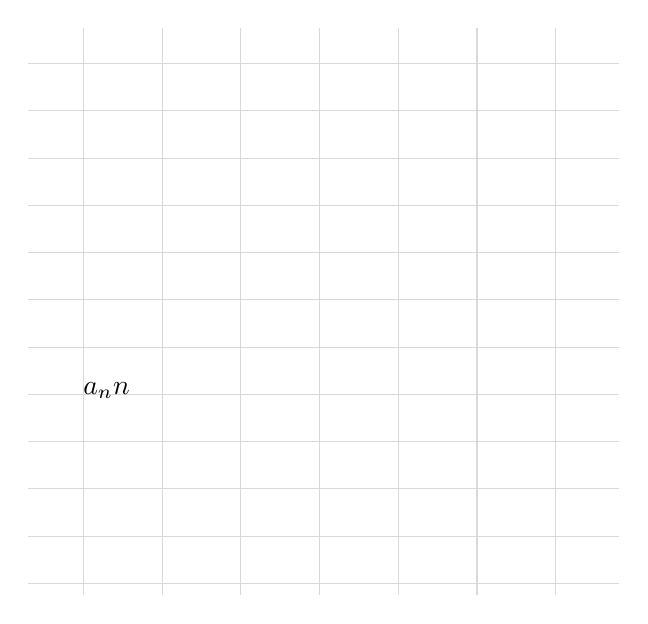
\begin{tikzpicture}[x=10mm, y=3mm]
\draw[xstep=1,ystep=2,color=gray!30] (-.7,-8.5) grid (6.8,15.5);
\tkzInit[xmin=-.7,xmax=6,xstep=1,ymin=-8.5,ymax=14.5,ystep=1]
\clip (-.7,-8.5) rectangle (6.8,15.5);
\begin{scope}[font=\small]
  \tkzLabelY[orig=false,step=2,label options={left=1pt}]
  \tkzDrawY[label=$a_n$]
  \tkzLabelX[orig=false,label options={below=1pt}]
  \tkzDrawX[label=$n$]
%  \node[below left] at (0,0) {$O$};
\end{scope}
\end{tikzpicture}

\end{center}
\end{esempio}
\end{exrig}
\vspazio\ovalbox{\risolvii \ref{ese:8a_succ.1}, \ref{ese:8a_succ.2}, \ref{ese:8a_succ.3}, \ref{ese:8a_succ.4}, \ref{ese:8a_succ.5}, \ref{ese:8a_succ.6}, \ref{ese:8a_succ.7}, \ref{ese:8a_succ.8}, \ref{ese:8a_succ.9}}


\section{Proprietà delle successioni}

Sulla base dei termini che le costituiscono, le successioni numeriche possono avere andamenti diversi tra loro ed avere quindi caratteristiche notevolmente differenti. Ad esempio, considerando il segno dei termini si ha che

\begin{definizione}
Una successione $\{a_n\}$ è detta
\begin{itemize*}
\item \emph{positiva} se $\forall n\in\insN_0\,$ si ha $a_n>0$;
\item \emph{negativa} se $\forall n\in\insN_0\,$ si ha $a_n<0$.
\end{itemize*} 
\end{definizione}

Può anche accadere che non tutti i termini di una successione siano positivi o negativi, ma che lo siano soltanto da un certo termine in poi. Si danno allora le seguenti definizioni

\begin{definizione}
Una successione $\{a_n\}$ è detta \emph{asintoticamente} (o \emph{definitivamente})
\begin{itemize*}
\item \emph{positiva} se $\exists \overline{n} : \forall n \in\insN_0$, $n > \overline{n}\,$ si ha $a_n>0$;
\item \emph{negativa} se $\exists \overline{n} : \forall n \in\insN_0$, $n > \overline{n}\,$ si ha $a_n<0$.
\end{itemize*} 
\end{definizione}

I termini di una successione, all'aumentare di $n$, possono avere inoltre un andamento crescente o decrescente, ovvero 

\begin{definizione}
Una successione $\{a_n\}$ è detta
\begin{itemize*}
\item \emph{crescente} se $\forall n\in\insN_0\,$ si ha $a_{n+1} > a_{n}$;
\item \emph{decrescente} se $\forall n\in\insN_0\,$ si ha $a_{n+1} < a_{n}$;
\item \emph{non decrescente} se $\forall n\in\insN_0\,$ si ha $a_{n+1} \geq a_{n}$;
\item \emph{non crescente} se $\forall n\in\insN_0\,$ si ha $a_{n+1} \leq a_{n}$;
\item \emph{costante} se $\forall n \in \insN_0\,$ si ha $a_{n+1} = k$.
\end{itemize*}
\end{definizione}

Tutte tali tipologie di successioni si dicono \emph{monotòne}.

In maniera analoga a quanto visto per il segno, nel caso in cui la successione sia crescente/{}decrescente/{}costante soltanto da un determinato $\overline{n}$ in poi, si parla di successione \emph{asintoticamente} (o \emph{definitivamente}) \emph{crescente}/{}\emph{decrescente}/{}\emph{costante}.

Dal punto di vista dei valori assunti dai termini della successione possiamo inoltre distinguere le successioni limitate da quelle non limitate, con la seguente definizione

\begin{definizione}
Una successione $\{a_n\}$ si dice 
\begin{itemize*}
\item \emph{limitata inferiormente} se $\exists m : a_n \geq m\; \forall n \in \insN_0$;
\item \emph{limitata superiormente} se $\exists M : a_n \leq M\; \forall n \in \insN_0$;
\item \emph{limitata} se $\exists M : \valass{a_n} \leq M\; \forall n \in \insN_0$.
\end{itemize*}
\end{definizione}

\begin{exrig}
\begin{esempio}
Determina l'andamento della successione $\{3\}$ e rappresentala sul piano cartesiano.

Il termine generico della successione è $a_n=3$ e quindi $a_1=3$, $a_2=3$, $a_3=3$, \ldots{} Si tratta di una successione positiva poiché $a_n=3>0$ e costante visto che $a_n$ è indipendente da $n$. Quindi è limitata poiché scelto, ad esempio, il valore 4, si ha $\valass{a_n}=3<4\; \forall n\in\insN_0$.
\begin{center}
 % (c) 2014 Daniele Masini - d.masini.it@gmail.com
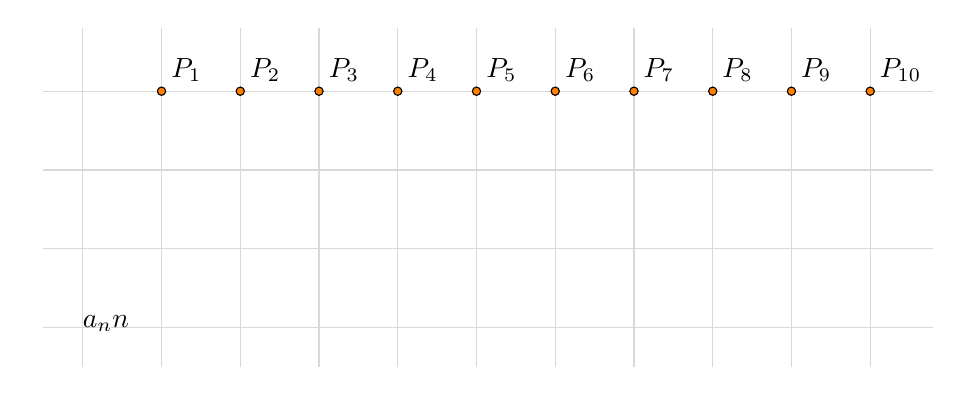
\begin{tikzpicture}[x=10mm, y=10mm]
\draw[xstep=1,ystep=1,color=gray!30] (-.5,-.5) grid (10.8,3.8);
\tkzInit[xmin=-.7,xmax=10,xstep=1,ymin=-.5,ymax=3,ystep=1]
\clip (-.7,-.7) rectangle (10.8,3.8);
\begin{scope}[font=\small]
  \tkzLabelY[orig=false,label options={left=1pt}]
  \tkzDrawY[label=$a_n$]
  \tkzLabelX[orig=false,label options={below=1pt}]
  \tkzDrawX[label=$n$]
%  \node[below left] at (0,0) {$O$};
\end{scope}
\foreach \x in {1,...,10}
{
  \draw[fill=orange] (\x,3) circle (1.5pt);
  \node[above right] at (\x,3) {$P_{\x}$};
}
\end{tikzpicture}

\end{center}
\end{esempio}

\begin{esempio}
Determina l'andamento della successione $\left\{n^2\right\}$ e rappresentala sul piano cartesiano.

Il termine generico della successione è $a_n=n^2$ e quindi $a_1=1$, $a_2=4$, $a_3=9$, \ldots{} Si tratta di una successione positiva poiché $n^2>0\;\forall n\in\insN_0$. Poiché inoltre $\forall n \in \insN_0\; n+1 > n$, per com'è definita l'elevazione a potenza si ha che $(n+1)^2 = n^2+2n+1 > n^2$ quindi la successione è crescente.
La successione è limitata inferiormente poiché positiva, cioè $a_n>0\;\forall n\in\insN_0$, ma non è limitata superiormente, infatti, supponiamo che lo sia, ovvero che $\exists M:\forall n>M$ risulti $n^2<M$. Si consideri $\overline{n}=M+1$ si ha che $\overline{n}^2=(M+1)^2=M^2+2M+1>M$ in contraddizione a quanto ipotizzato.
\begin{center}
 % (c) 2014 Daniele Masini - d.masini.it@gmail.com
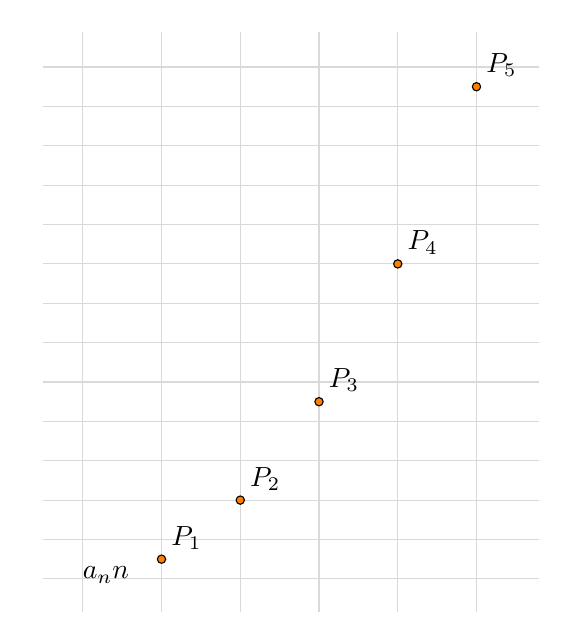
\begin{tikzpicture}[x=10mm, y=2.5mm]
\draw[xstep=1,ystep=2,color=gray!30] (-.5,-1.7) grid (5.8,27.8);
\tkzInit[xmin=-.7,xmax=5,xstep=1,ymin=-.5,ymax=26.2,ystep=1]
\clip (-.7,-1.7) rectangle (5.8,28);
\begin{scope}[font=\small]
  \tkzLabelY[orig=false,step=2,label options={left=1pt}]
  \tkzDrawY[label=$a_n$]
  \tkzLabelX[orig=false,label options={below=1pt}]
  \tkzDrawX[label=$n$]
%  \node[below left] at (0,0) {$O$};
\end{scope}
\foreach \x in {1,...,5}
{
  \draw[fill=orange] (\x,{\x*\x}) circle (1.5pt);
  \node[above right] at (\x,{\x*\x}) {$P_{\x}$};
}
\end{tikzpicture}

\end{center}
\end{esempio}

\begin{esempio}
Determina l'andamento della successione $\left\{\dfrac{3n^2-5}{n^2+1}\right\}$ e rappresentala sul piano cartesiano.

Il termine generico della successione è $a_n = \dfrac{3n^2-5}{n^2+1}$ e quindi $a_1=-1$, $a_2=\dfrac{7}{5}$, $a_3=\dfrac{7}{5}$, $a_4=\dfrac{43}{17}$, \ldots{} La successione non è positiva, né negativa, ma è definitivamente positiva in quanto il denominatore è sempre positivo ed il numeratore $3n^2-5 > 0 \:\Rightarrow\: n>\sqrt{\frac{5}{3}}$. Vediamo che andamento ha la successione
\[a_n = \dfrac{3n^2-5}{n^2+1}\qquad\text{e}\qquad a_{n+1} = \dfrac{3(n+1)^2-5}{(n+1)^2+1} = \dfrac{3n^2+6n+3-5}{n^2+2n+1+1} = \dfrac{3n^2+6n-2}{n^2+2n+2}.\]
I denominatori sono entrambi sempre positivi (sono addizioni di termini positivi). Portiamo le frazioni allo stesso denominatore e analizziamo i numeratori:
\[a_n = \dfrac{(3n^2-5)(n^2+2n+2)}{(n^2+1)(n^2+2n+2)} = \dfrac{3n^4+6n^3+n^2-10n-10}{(n^2+1)(n^2+2n+2)}\]
e
\[a_{n+1} = \dfrac{(n^2+1)(3n^2+6n-2)}{(n^2+1)(n^2+2n+2)} = \dfrac{3n^4+6n^3+n^2+6n-2}{(n^2+1)(n^2+2n+2)}.\]
Adesso facciamo la differenza tra i numeratori (il denominatore è lo stesso):
\[N(a_{n+1}) - N(a_n) = 3n^4+6n^3+n^2+6n-2 - \left(3n^4+6n^3+n^2-10n-10\right) = 16n+8.\]
Quindi, poiché $n>0$ si ha che $16n+8>0\; \forall n \in \insN_0$, cioè $a_{n+1} > a_n$. Quindi la successione è crescente.
\begin{center}
 % (c) 2014 Daniele Masini - d.masini.it@gmail.com
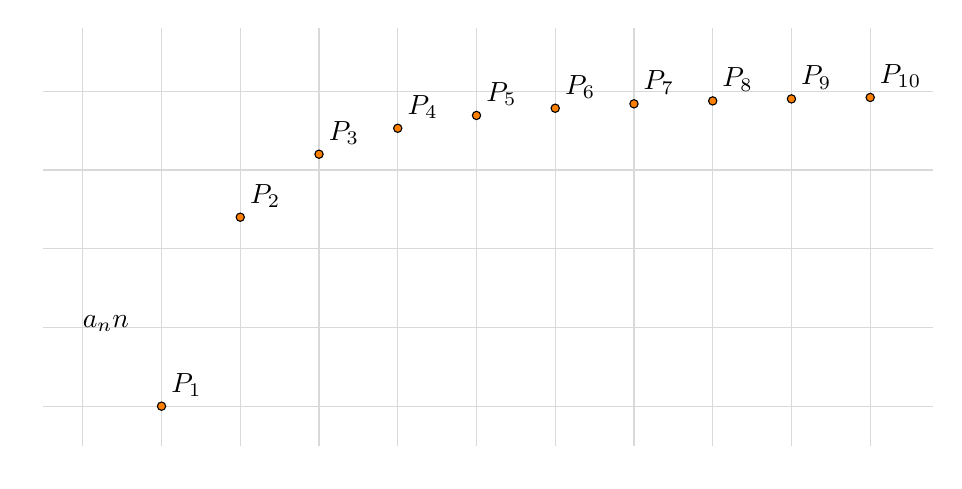
\begin{tikzpicture}[x=10mm, y=10mm]
\draw[xstep=1,ystep=1,color=gray!30] (-.5,-1.5) grid (10.8,3.8);
\tkzInit[xmin=-.7,xmax=10,xstep=1,ymin=-1.5,ymax=3,ystep=1]
\clip (-.7,-1.7) rectangle (10.8,3.8);
\begin{scope}[font=\small]
  \tkzLabelY[orig=false,label options={left=1pt}]
  \tkzDrawY[label=$a_n$]
  \tkzLabelX[orig=false,label options={below=1pt}]
  \tkzDrawX[label=$n$]
%  \node[below left] at (0,0) {$O$};
\end{scope}
\foreach \x in {1,...,10}
{
  \draw[fill=orange] (\x,{(3*\x*\x-5)/(\x*\x+1)}) circle (1.5pt);
  \node[above right] at (\x,{(3*\x*\x-5)/(\x*\x+1)}) {$P_{\x}$};
}
\end{tikzpicture}

\end{center}
\end{esempio}

\begin{esempio}
Determina l'andamento della successione $\left\{\dfrac{\sqrt{7n^2-2n+1}}{n^2+3}\right\}$  e rappresentala sul piano cartesiano.

Il termine generico della successione è $a_n = \dfrac{\sqrt{7n^2-2n+1}}{n^2+3}$ e quindi $a_1=\dfrac{\sqrt{6}}{4}$, $a_2=\dfrac{5}{7}$, $a_3=\dfrac{\sqrt{58}}{12}$, \ldots{} è positiva in quanto sono positivi sia il denominatore (è la somma di un quadrato e di un numero positivo) che il numeratore, poiché $7n^2-2n+1$ ha $\Delta < 0$.
Vediamo che andamento ha la successione:
\[a_n = \dfrac{\sqrt{7n^2-2n+1}}{n^2+3}\qquad\text{e}\qquad a_{n+1} = \dfrac{\sqrt{7(n+1)^2-2(n+1)+1}}{(n+1)^2+3} = \dfrac{\sqrt{7n^2+12n+6}}{n^2+2n+4}\]
eleviamoli al quadrato (tanto per il confronto si ha che $a_n>a_{n+1} \:\Leftrightarrow\: {a_n}^2>{a_{n+1}}^2$, cioè la relazione d'ordine tra $a_n$ e $a_{n+1}$ non cambia elevandoli al quadrato) e portandoli entrambi allo stesso denominatore si ha
\[a_n = \dfrac{(7n^2-2n+1)(n^2+2n+4)^2}{(n^2+3)^2(n^2+2n+4)^2} = \dfrac{7n^6+26n^5+77n^4+92n^3+92n^2−16n+16}{(n^2+3)^2(n^2+2n+4)^2}\]
e
\[a_{n+1} = \dfrac{(n^2+n+1)(n^2+3)^2}{(n^2+3)^2(n^2+2n+4)^2} = \dfrac{7n^6+12n^5+48n^4+72n^3+99n^2+108n+54}{(n^2+3)^2(n^2+2n+4)^2}\]
Adesso facciamo la differenza tra i numeratori:
\begin{align*}
N(a_{n+1})-N(a_n)&=7n^6+12n^5+48n^4+72n^3+99n^2+108n+54+\\ &\phantom{=\,}-\left(7n^6+26n^5+77n^4+92n^3+92n^2−16n+16\right)\\
&=-14n^5-29n^4-20n^3+7n^2+124n+38.
\end{align*}
Per calcolare il valore di $n$ per il quale tale quantità risulta positiva, bisogna risolvere la disequazione $-14n^5-29n^4-20n^3+7n^2+124n+38>0$. A noi non interessa trovare il valore di $n$, ma ci accontentiamo di sapere se da un determinato $\overline{n}$ in poi la quantità risulta positiva o negativa. Per valutarlo, mettiamo in evidenza la variabile con esponente più elevato, cioè $n^5$:
\[N(a_{n+1})-N(a_n)=n^5\left(-14-\frac{29}{n}-\frac{20}{n^2}+\frac{7}{n^3}+\frac{124}{n^4}+\frac{38}{n^5}\right)\]
e osserviamo che per $n$ molto grande tutti i termini che hanno $n$ al denominatore diventano sempre più piccoli e quindi insignificanti sia rispetto ai valori costanti, come 14, sia rispetto a $n^5$. Pertanto, per $n$ molto grande tale quantità varrà circa $-14n^5$ e quindi avrà il suo segno, cioè sarà negativa, ovvero $a_{n+1}<a_n$. Dunque la successione è definitivamente decrescente.
\begin{center}
 % (c) 2014 Daniele Masini - d.masini.it@gmail.com
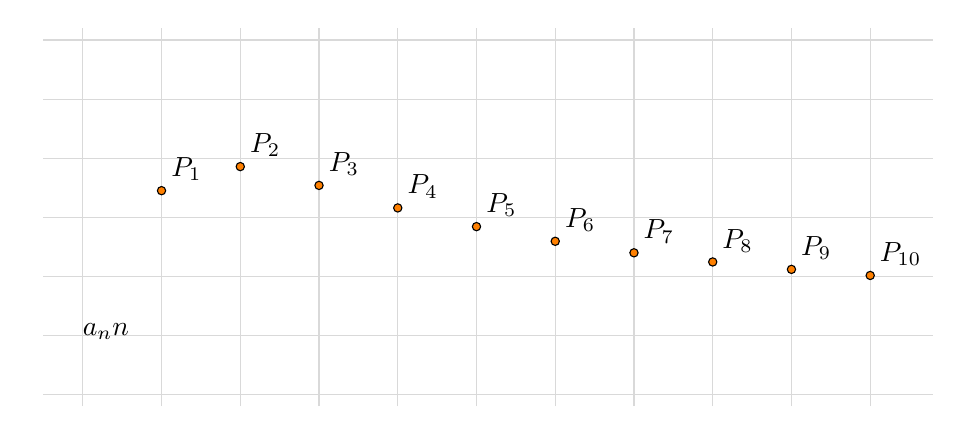
\begin{tikzpicture}[x=10mm, y=30mm]
\draw[xstep=1,ystep=.25,color=gray!30] (-.5,-.3) grid (10.8,1.3);
\tkzInit[xmin=-.7,xmax=10,xstep=1,ymin=-.3,ymax=0.7,ystep=1]
\clip (-.7,-.3) rectangle (10.8,1.3);
\begin{scope}[font=\small]
  \tkzLabelY[orig=false,label options={left=1pt}]
  \tkzDrawY[label=$a_n$]
  \tkzLabelX[orig=false,label options={below=1pt}]
  \tkzDrawX[label=$n$]
%  \node[below left] at (0,0) {$O$};
\end{scope}
\foreach \x in {1,...,10}
{
  \draw[fill=orange] (\x,{(7*\x*\x-2*\x+1)^(1/2)/(\x*\x+3)}) circle (1.5pt);
  \node[above right] at (\x,{(7*\x*\x-2*\x+1)^(1/2)/(\x*\x+3)}) {$P_{\x}$};
}
\end{tikzpicture}

\end{center}
\end{esempio}
\end{exrig}
\vspazio\ovalbox{\risolvii \ref{ese:8a_psucc.1}, \ref{ese:8a_psucc.2}, \ref{ese:8a_psucc.3}, \ref{ese:8a_psucc.4}, \ref{ese:8a_psucc.5}}

\section{Limite di una successione}

Consideriamo la successione $\left\{\dfrac{n-1}{n+1}\right\}$.

Si tratta di una successione non negativa poiché il denominatore è positivo e il numeratore $n-1\ge0\;\forall n\in\insN_0$. Inoltre la successione è crescente, infatti $a_1=0$, $a_2=\dfrac{1}{3}$, $a_3=\dfrac{1}{2}$, $a_4=\dfrac{3}{5}$, $a_5=\dfrac{2}{3}$, \ldots{} In generale
\[a_n = \frac{n-1}{n+1}\qquad\text{e}\qquad a_{n+1} = \frac{n+1-1}{n+1+1}=\frac{n}{n+2}\]
portando tutto allo stesso denominatore
\[a_n=\frac{(n-1)(n+2)}{(n+1)(n+2)}=\frac{n^2+n-2}{(n+1)(n+2)}\]
e
\[a_{n+1}=\frac{n(n+1)}{(n+2)(n+1)}=\frac{n^2+n}{(n+2)(n+1)}\]
quindi per qualunque $n$ si ha $a_{n+1} > a_n$, ovvero la successione è crescente.

Possiamo però osservare che per quanto grande diventi $n$, il numeratore $n-1$ non sarà mai maggiore del denominatore $n+1$, pertanto $a_n$ non supererà mai il valore 1. La successione cresce rimanendo sempre minore di 1 e quindi il valore di $a_n$ vi si avvicinerà sempre di più senza mai raggiungerlo, ovvero lo raggiungerà per $n$ infinitamente grande. Diremo in tal caso che 1 è il limite della successione, ovvero che $a_n$ tende ad 1 per $n$ che tende all'infinito.

Il \emph{limite} di una successione $\{a_n\}$ è il valore $L$ che $a_n$ tende ad assumere quando $n$ diventa molto grande, cioè quando $n$ tende all'infinito. Matematicamente si scrive

\[\lim_{n\to+\infty} a_n = L.\]

Sulla base di questa caratteristica, esistono successioni il cui valore non è limitato, ovvero crescono all'infinito (o decrescono all'infinito in senso negativo) e si dicono \emph{divergenti}, mentre quelle che hanno un limite si dicono \emph{convergenti}. Esistono anche successioni limitate ma che non tendono a un valore ben definito e quindi non sono né convergenti né divergenti. Queste ultime sono dette \emph{oscillanti}.

\begin{exrig}
\begin{esempio}
Determina l'andamento e il limite della successione armonica $\left\{\dfrac{1}{n}\right\}$.

Si tratta di una successione a termini positivi, in quanto $\dfrac{1}{n}>0\;\forall n\in\insN_0$ e decrescente, infatti $a_n=\dfrac{1}{n}$ e $a_{n+1}=\dfrac{1}{n+1}$. Rappresentando i due termini con lo stesso denominatore:
\[a_n=\dfrac{n+1}{n(n+1)}\qquad\text{e}\qquad a_{n+1}=\dfrac{n}{n(n+1)}\]
da cui si deduce immediatamente che $a_{n+1}<a_n\;\forall n \in \insN_0$.

Al crescere di $n$ il valore $\dfrac{1}{n}$ diventa sempre più piccolo fino a confondersi con lo 0 per $n$ tendente all'infinito. Quindi il limite della successione è 0, ovvero la successione converge a 0 e si scrive
\[\lim_{n\to+\infty} \dfrac{1}{n} = 0.\]
\end{esempio}

\begin{esempio}
Determina l'andamento e il limite della successione $\left\{\sqrt{n+1}\right\}$.

Si tratta di una successione a termini positivi, in quanto $n+1>0\;\forall n\in\insN_0$. La successione è crescente poiché $a_n=\sqrt{n+1}$ e $a_{n+1}=\sqrt{n+2}$ e quindi $a_n < a_{n+1}\;\forall n\in\insN_0$. 

Al crescere di $n$ il valore $\sqrt{n+1}$ diventa sempre più grande. Quindi la successione non è limitata, pertanto per $n$ tendente all'infinito la successione tende ad infinito, cioè è divergente, ovvero
\[\lim_{n\to+\infty} \sqrt{n+1} = +\infty.\]

\end{esempio}

\begin{esempio}
Determina l'andamento e il limite della successione $\left\{(-1)^n\right\}$.

La successione ha termini di segno altalenante, cioè $a_1 = (-1)^1 = -1$, $a_2 = (-1)^2 = 1$, $a_3 = (-1)^3 = -1$, $a_4 = (-1)^4 = 1$, $a_5 = (-1)^5 = -1$, \ldots{} cioè con $n$ pari i termini sono positivi e con $n$ dispari negativi. La successione è limitata, infatti è sufficiente prendere il valore 2 e si ha che $\valass{(-1)^n}=1<2\;\forall n\in\insN_0$.

Al crescere di $n$ il valore $(-1)^n$ non è definito poiché non è chiaro se assume il valore 1 o $-1$. Quindi la successione è oscillante ed il limite non esiste, ovvero si scrive
\[\lim_{n\to+\infty} (-1)^n = \nexists.\]
\end{esempio}

\begin{esempio}
Determina l'andamento ed il limite della successione $\left\{\dfrac{2n^2-3}{n^2+n+1}\right\}$.

La successione ha termini di segno positivo poiché sia il numeratore che il denominatore di $a_n$ sono positivi $\forall n\in\insN_0$.

Per quanto riguarda l'andamento si ha:
\[a_n=\frac{2n^2-3}{n^2+n+1}\qquad\text{e}\qquad a_{n+1}=\frac{2(n+1)^2-3}{(n+1)^2+(n+1)+1}=\frac{2n^2+4n-1}{n^2+3n+3}\]
e portando allo stesso denominatore
\[a_n=\frac{(2n^2-3)(n^2+3n+3)}{(n^2+n+1)(n^2+3n+3)}=\frac{2n^4+6n^3+3n^2−9n−9}{(n^2+n+1)(n^2+3n+3)}\]
e
\[a_{n+1}=\frac{(2n^2+4n-1)(n^2+n+1)}{(n^2+n+1)(n^2+3n+3)}=\frac{2n^4+6n^3+5n^2+3n−1}{(n^2+n+1)(n^2+3n+3)}.\]
Considerando i numeratori e facendone la differenza si ha:
\[N(a_{n+1})-N(a_n) = 2n^4+6n^3+5n^2+3n−1 - (2n^4+6n^3+3n^2−9n−9) = 2n^2+12n+8.\]
che è un valore sempre positivo per $n\in\insN_0$, ovvero $a_{n+1}>a_n$, pertanto la successione è crescente.

Per determinare il limite, consideriamo il termine generico e mettiamo in evidenza sia al numeratore che al denominatore la massima potenza alla quale compare $n$, si ha:
\[a_n=\dfrac{2n^2-3}{n^2+n+1}=\dfrac{\cancel{n^2}\left(2-\dfrac{3}{n^2}\right)}{\cancel{n^2}\left(1+\dfrac{1}{n}+\dfrac{1}{n^2}\right)}.\]
Osserviamo che quando $n$ tende all'infinito i termini nei quali $n$ compare al denominatore tendono a 0 e quindi il rapporto diventa $\dfrac{2}{1}=2$ che è il valore al quale converge la successione, ovvero
\[\lim_{n\to+\infty} \dfrac{2n^2-3}{n^2+n+1} = 2.\]
\end{esempio}

\begin{esempio}
Determina il limite della successione $\left\{n-\sqrt{n^2-3n+2}\right\}$.

Per $n$ molto grande sia la prima parte del termine generico ($n$) che la parte sotto radice tendono a $+\infty$ e quindi la loro differenza tende ad un valore $+\infty - \infty$ indeterminato. Il simbolo $\infty$, infatti, non è un numero, e quindi per esso non valgono le regole delle operazioni, pertanto non è detto che $+\infty - \infty = 0$. Per determinare il limite della successione è necessario scrivere il suo termine generico $a_n$ in un'altra forma.

Ricordando il prodotto notevole $(a-b)(a+b) = a^2-b^2$, eliminiamo (al numeratore) la radice quadrata moltiplicando e dividendo $a_n$ per $n+\sqrt{n^2-3n+2}$
\[a_n=\frac{\left(n-\sqrt{n^2-3n+2}\right)\left(n+\sqrt{n^2-3n+2}\right)}{n+\sqrt{n^2-3n+2}}= \frac{n^2-\left(n^2-3n+2\right)}{n+\sqrt{n^2-3n+2}}=\frac{3n-2}{n+\sqrt{n^2-3n+2}}.\]
Quindi mettiamo in evidenza il termine $n$
\[a_n=\frac{\cancel{n}\left(3-\dfrac{2}{n}\right)}{\cancel{n}\left(1+\sqrt{1-\dfrac{3}{n}+\dfrac{2}{n^2}}\right)}=
\frac{3-\dfrac{2}{n}}{1+\sqrt{1-\dfrac{3}{n}+\dfrac{2}{n^2}}}.\]

Per $n$ che tende all'infinito, si ha che i termini che hanno al denominatore $n$, o una sua potenza, tendono a 0, quindi $a_n$ tende a $\dfrac{3}{1+\sqrt{1}} = \dfrac{3}{2}$. Pertanto si può scrivere
\[\lim_{n\to+\infty} n-\sqrt{n^2-3n+2} = \frac{3}{2}.\]
\end{esempio}

\end{exrig}
\vspazio\ovalbox{\risolvii \ref{ese:8a_lsucc.1}, \ref{ese:8a_lsucc.2}, \ref{ese:8a_lsucc.3}, \ref{ese:8a_lsucc.4}, \ref{ese:8a_lsucc.5}, \ref{ese:8a_lsucc.6}, \ref{ese:8a_lsucc.7}}


\section{Progressioni}

Esistono alcune successioni dotate di particolari proprietà, come le progressioni aritmetiche e geometriche, descritte di seguito.

\subsection{Progressione aritmetica}

\begin{definizione}
Si definisce \emph{progressione aritmetica} una successione $\{a_n\}$ nella quale la differenza tra due termini consecutivi è costante, cioè $a_{n+1} - a_n = q$, e il valore $q$ è detto \emph{ragione} della progressione.
\end{definizione}

Poiché in una progressione aritmetica ogni termine si ottiene dal precedente incrementandolo della ragione $q$ si ha che
\[a_n = a_{n-1}+q = a_{n-2}+2q = \ldots = a_1 + (n-1)q\]
cioè il termine $n$-esimo si ricava direttamente conoscendo il primo termine e la ragione.

\`E evidente che una progressione aritmetica risulta limitata o meno dipendentemente dal valore della sua ragione $q$. Infatti se $q>0$ la progressione sarà crescente e tenderà a $+\infty$, se invece $q<0$ la progressione sarà decrescente e tenderà a $-\infty$. Infine, se $q=0$ la progressione è costante e pari a $a_1$.

Consideriamo la progressione aritmetica $\{1$, 2, 3, 4, $\ldots\}$, di ragione 1 con $a_1=1$ e calcoliamone la somma $S_n$ dei primi $n$ termini.
\[S_1=1\text{,}\quad S_2=1+2=3\text{,}\quad S_3=1+2+3=6\text{,}
\quad S_4=1+2+3+4=10\text{,}\quad\ldots\]

Cerchiamo dunque una formula per calcolare $S_n$. Scriviamolo per esteso:
\[S_n = a_1 + a_2 + a_3 + \ldots + a_{n-2} + a_{n-1} + a_n = 1 + 2 + 3 + \ldots + (n-2) + (n-1) + n.\]
Aggiungiamoci $S_n$ e sommiamo i termini della prima $S_n$ con quelli della seconda $S_n$ presi nell'ordine opposto, cioè
\begin{align*}
2S_n &= \underbrace{1 + 2 + 3 + \ldots + (n-2) + (n-1) + n}_{n\text{ elementi (}=S_n\text{)}} + \underbrace{n + (n-1) + (n-2) + \ldots + 3 + 2 + 1}_{n\text{ elementi (}=S_n\text{)}}\\
&=\underbrace{(1 + n) + [2 + (n-1)] + [3 + (n-2)] + \ldots + [(n-2) + 3] + [(n-1) + 2] + (n + 1)}_{n\text{ elementi}}\\
&=\underbrace{(n + 1) + (n + 1) + (n + 1) + \ldots + (n + 1) + (n + 1) + (n + 1)}_{n\text{ elementi}}\\
&=n(n+1).
\end{align*}
Quindi
\[S_n = \frac{n(n+1)}{2}.\]

Generalizziamo il risultato trovato.

Consideriamo la generica progressione aritmetica $\{a_n\}$ di ragione $q$ e calcoliamone la somma $S_n$ dei primi $n$ termini.
\begin{align*}
S_n &= \sum_{i=1}^{n}a_i=a_1+a_2+a_3+\ldots+a_n\\
&=a_1+(a_1+q)+(a_1+2q)+\ldots+[a_1+(n-1)q]\\
&=na_1+q[1+2+\ldots+(n-1)].
\end{align*}
Dal risultato precedente sappiamo che $1+2+\ldots+(n-1)=S_{n-1}=\dfrac{(n-1)n}{2}$, quindi sostituendolo si ha
\[S_n=na_1+q\frac{(n-1)n}{2}=\frac{n}{2}[2a_1+q(n-1)]=\frac{n}{2}[a_1+a_1+q(n-1)]=\frac{n}{2}(a_1+a_n).\]

Il procedimento precedentemente utilizzato per trovare $S_n$ non pone vincoli sugli estremi, quindi la formula vale qualunque siano $a_1$ e $a_n$. Quindi, se consideriamo i $k$ termini consecutivi di una progressione aritmetica da $a_n$ ad $a_{n+k-1}$ la loro somma è data da $\dfrac{k}{2}(a_n+a_{n+k-1})$. Ricordando la formula della media aritmetica, si può dunque dire che la somma dei termini di una porzione di una progressione aritmetica è la media dei due estremi moltiplicata per il numero dei termini considerati (estremi inclusi).

\vspazio\ovalbox{\risolvii \ref{ese:8a_progr.1}, \ref{ese:8a_progr.2}, \ref{ese:8a_progr.3}, \ref{ese:8a_progr.4}, \ref{ese:8a_progr.5}, \ref{ese:8a_progr.6}, \ref{ese:8a_progr.7}, \ref{ese:8a_progr.8}, \ref{ese:8a_progr.8}, \ref{ese:8a_progr.9}, \ref{ese:8a_progr.10},}

\ovalbox{\ref{ese:8a_progr.11}, \ref{ese:8a_progr.12}, \ref{ese:8a_progr.13}, \ref{ese:8a_progr.14}, \ref{ese:8a_progr.15}, \ref{ese:8a_progr.16}, \ref{ese:8a_progr.17}, \ref{ese:8a_progr.18}, \ref{ese:8a_progr.19}, \ref{ese:8a_progr.20}, \ref{ese:8a_progr.21}}


\subsection{Progressione geometrica}

\begin{definizione}
Si definisce \emph{progressione geometrica} una successione $\{a_n\}$ nella quale il rapporto tra due termini consecutivi è costante, cioè $\dfrac{a_{n+1}}{a_n} = q$, e il valore $q$ è detto \emph{ragione} della progressione.
\end{definizione}

Poiché in una progressione geometrica ogni termine si ottiene dal precedente moltiplicandolo per la ragione $q$ si ha che
\[a_n = a_{n-1}q = a_{n-2}q^2 = \ldots = a_1 q^{n-1}\]
cioè il termine $n$-esimo si ricava direttamente conoscendo il primo termine e la ragione.

Una progressione geometrica risulta limitata o meno dipendentemente dal valore della sua ragione $q$ e dal segno di $a_1$. Considerando il caso in cui $a_1>0$, l'andamento della serie è quello riportato nella seguente tabella
\begin{center}
\begin{tabular}{cl}
\toprule
Ragione & Andamento\\
\midrule
$q>1$ & crescente (divergente)\\
$q=1$ & costante (convergente)\\
$0<q<1$ & decrescente (convergente)\\
$q=0$ & decrescente (convergente)\\
$-1<q<0$ & decrescente in valore assoluto (convergente)\\
$q=-1$ & limitata (oscillante)\\
$q<-1$ & crescente in valore assoluto (divergente)\\
\bottomrule
\end{tabular}
\end{center}
Il caso in cui $a_1<0$ è il simmetrico rispetto a quello riportato nella tabella precedente.

Consideriamo la generica progressione geometrica $\{a_n\}$ di ragione $q$ e calcoliamo la somma $S_n$ dei primi $n$ termini.
\begin{align*}
S_n&=\sum_{i=1}^{n}a_i=a_1+a_2+a_3+\ldots+a_{n-1}+a_n\\
&=a_1+\left(a_1q\right)+\left(a_1q^2\right)+\ldots+\left(a_1q^{n-2}\right)+\left(a_1q^{n-1}\right)\\
&=a_1\left(1+q+q^2+\ldots+q^{n-2}+q^{n-1}\right).
\end{align*}
Moltiplichiamo per $1-q$ (con $q \ne 1$, se $q=1$ la progressione è costante, cioè $a_n=a_1\;\forall n\in\insN_0$ e $S_n = na_1$), si ha
\begin{align*}
S_n(1-q)&=a_1(1-q)\left(1+q+q^2+\ldots+q^{n-1}\right)\\
&=a_1\left(1+q+q^2+\ldots+q^{n-1}-q-q^2-q^3-\ldots-q^n\right)\\
&=a_1\left(1+\cancel{q}+\cancel{q^2}+\cancel{\ldots\vphantom{q^n}}+\cancel{q^{n-1}}-\cancel{q}-\cancel{q^2}-\cancel{q^3}-\cancel{\ldots\vphantom{q^n}}-q^n\right)\\
&=a_1\left(1-q^n\right).
\end{align*}
Quindi (se $q\ne 1$) si ha
\[S_n=a_1\frac{1-q^n}{1-q}=a_1\frac{q^n-1}{q-1}.\]

\ovalbox{\risolvii \ref{ese:8a_progr.22}, \ref{ese:8a_progr.23}, \ref{ese:8a_progr.24}, \ref{ese:8a_progr.25}, \ref{ese:8a_progr.26}, \ref{ese:8a_progr.27}, \ref{ese:8a_progr.28}, \ref{ese:8a_progr.29}, \ref{ese:8a_progr.30}, \ref{ese:8a_progr.31}, \ref{ese:8a_progr.32},}

\ovalbox{\ref{ese:8a_progr.33}}

\newpage

% (c) 2014 Daniele Masini - d.masini.it@gmail.com
\section{Esercizi}
\subsection{Esercizi dei singoli paragrafi}
\subsubsection*{\thechapter.1 - Successioni numeriche}

\begin{esercizio}
\label{ese:8a_succ.1}
Le due scritture
\[1\text{, }\frac{1}{2}\text{, }\frac{1}{3}\text{, }\frac{1}{4}\text{, }\frac{1}{5}\text{, }\frac{1}{6}\text{, }\ldots \qquad
1\text{, }\frac{1}{3}\text{, }\frac{1}{5}\text{, }\frac{1}{4}\text{, }\frac{1}{2}\text{, }\frac{1}{6}\text{, }\ldots\]
rappresentano la stessa successione? Perché?
\end{esercizio}

\begin{esercizio}
\label{ese:8a_succ.2}
Scrivere il termine generico $a_n$ della successione $\dfrac{1}{3}$, $\dfrac{1}{6}$, $\dfrac{1}{9}$, $\dfrac{1}{12}$, \ldots{}
\end{esercizio}

\begin{esercizio}
\label{ese:8a_succ.3}
Scrivere il termine generico $a_n$ della successione $\dfrac{1}{2}$, $-\dfrac{1}{2}$, $\dfrac{1}{2}$, $-\dfrac{1}{2}$, \ldots{}
\end{esercizio}

\begin{esercizio}
\label{ese:8a_succ.4}
Scrivere il termine generico $a_n$ della successione $\dfrac{1}{2}$, $\dfrac{3}{5}$, $\dfrac{5}{8}$, $\dfrac{7}{11}$, $\dfrac{9}{14}$, \ldots{}
\end{esercizio}

\begin{esercizio}
\label{ese:8a_succ.5}
Scrivere il termine generico $a_n$ della successione $\sqrt{2}-1$, $\sqrt{6}-2$, $2\sqrt{3}-3$, $2\sqrt{5}-4$, \ldots{}
\end{esercizio}

\begin{esercizio}
\label{ese:8a_succ.6}
Si determini il dominio della successione $\left\{\dfrac{2n-1}{3n-1}\right\}$ e si rappresentino i suoi primi 5 termini sul piano cartesiano.
\end{esercizio}

\begin{esercizio}
\label{ese:8a_succ.7}
Si determini il dominio della successione $\left\{\dfrac{4n-5}{2n-4}\right\}$ e si rappresentino i suoi primi 5 termini sul piano cartesiano.
\end{esercizio}

\begin{esercizio}
\label{ese:8a_succ.8}
Si determini il dominio della successione $\left\{\dfrac{n-3}{2n-3}\right\}$ e si rappresentino i suoi primi 5 termini sul piano cartesiano.
\end{esercizio}

\begin{esercizio}
\label{ese:8a_succ.9}
Si determini il dominio della successione $\left\{\dfrac{n^2-1}{n}\right\}$ e si rappresentino i suoi primi 5 termini sul piano cartesiano.
\end{esercizio}

\subsubsection*{\thechapter.2 - Proprietà delle successioni}

\begin{esercizio}
\label{ese:8a_psucc.1}
Determina l'andamento della successione $\left\{3-\sqrt{n}\right\}$ e rappresenta i suoi primi 5 termini sul piano cartesiano.
\end{esercizio}

\begin{esercizio}
\label{ese:8a_psucc.2}
Determina l'andamento della successione $\left\{\sqrt{1+n}\right\}$ e rappresenta i suoi primi 5 termini sul piano cartesiano.
\end{esercizio}

\begin{esercizio}
\label{ese:8a_psucc.3}
Determina l'andamento della successione $\left\{\dfrac{n^2-1}{n}\right\}$ e rappresenta i suoi primi 5 termini sul piano cartesiano.
\end{esercizio}

\begin{esercizio}
\label{ese:8a_psucc.4}
Determina l'andamento della successione $\left\{(-1)^{2n}\right\}$ e rappresenta i suoi primi 5 termini sul piano cartesiano.
\end{esercizio}

\begin{esercizio}
\label{ese:8a_psucc.5}
Determina l'andamento della successione $\left\{(-1)^{3n}\right\}$ e rappresenta i suoi primi 5 termini sul piano cartesiano.
\end{esercizio}


\subsubsection*{\thechapter.3 - Limite di una successione}

\begin{esercizio}
\label{ese:8a_lsucc.1}
Determina, se esiste, il limite della successione $\left\{\dfrac{3n-1}{2n-1}\right\}$.
\end{esercizio}

\begin{esercizio}
\label{ese:8a_lsucc.2}
Determina, se esiste, il limite della successione $\left\{\dfrac{n^2}{n^2-1}\right\}$.
\end{esercizio}

\begin{esercizio}
\label{ese:8a_lsucc.3}
Determina, se esiste, il limite della successione $\left\{\dfrac{n+1}{2n^2}\right\}$.
\end{esercizio}

\begin{esercizio}
\label{ese:8a_lsucc.4}
Determina, se esiste, il limite della successione $\left\{\dfrac{5n^3-4}{n^2-n^3}\right\}$.
\end{esercizio}

\begin{esercizio}
\label{ese:8a_lsucc.5}
Determina, se esiste, il limite della successione $\left\{(-1)^{3n}\right\}$.
\end{esercizio}

\begin{esercizio}
\label{ese:8a_lsucc.6}
Determina, se esiste, il limite della successione $\left\{\sqrt{n^2+5n}-n\right\}$.
\end{esercizio}

\begin{esercizio}
\label{ese:8a_lsucc.7}
Determina, se esiste, il limite della successione $\left\{\dfrac{n^2+1}{n-\sqrt{n}}\right\}$.
\end{esercizio}


\subsubsection*{\thechapter.4 - Progressioni}

\begin{esercizio}
\label{ese:8a_progr.1}
Scrivi i primi 5 termini di una progressione aritmetica con $a_1=4$ e ragione $q=3$. Quindi rappresentali sul piano cartesiano.
\end{esercizio}

\begin{esercizio}
\label{ese:8a_progr.2}
Scrivi i primi 5 termini di una progressione aritmetica con $a_1=\frac{3}{2}$ e ragione $q=\frac{1}{2}$. Quindi rappresentali sul piano cartesiano.
\end{esercizio}

\begin{esercizio}
\label{ese:8a_progr.3}
Calcolare la ragione $q$ e scrivere altri 3 termini della seguente successione aritmetica: $-4$, $-1$, $2$, $5$, \ldots{} Quindi li si rappresenti sul piano cartesiano.
\end{esercizio}

\begin{esercizio}
\label{ese:8a_progr.4}
Calcolare la ragione $q$ e scrivere altri 3 termini della seguente successione aritmetica: $\frac{4}{5}$, 1, $\frac{6}{5}$, $\frac{7}{5}$, \ldots{} Quindi li si rappresenti sul piano cartesiano.
\end{esercizio}

\begin{esercizio}
\label{ese:8a_progr.5}
Calcolare la ragione $q$ e scrivere altri 3 termini della seguente successione aritmetica: $\frac{2\sqrt{3}}{5}$, $\frac{7\sqrt{3}}{5}$, $\frac{4\cdot3^{\frac{3}{2}}}{5}$, $\frac{17\sqrt{3}}{5}$, \ldots{} Quindi li si rappresenti sul piano cartesiano.
\end{esercizio}

\begin{esercizio}
\label{ese:8a_progr.6}
Di una progressione aritmetica sono assegnati $a_1=3$ e la ragione $q=4$. Calcolare $a_9$ e $a_{15}$.
\end{esercizio}

\begin{esercizio}
\label{ese:8a_progr.7}
Di una progressione aritmetica sono assegnati $a_1=-\frac{3}{5}$ e $a_8=\frac{18}{5}$. Calcolare la ragione $q$.
\end{esercizio}

\begin{esercizio}
\label{ese:8a_progr.8}
Di una progressione aritmetica si conoscono $a_2=7$ e la ragione $q=\frac{3}{4}$. Calcolare $a_8$.
\end{esercizio}

\begin{esercizio}
\label{ese:8a_progr.9}
Di una progressione aritmetica si conoscono $a_3=\frac{3}{5}$ e $a_8=\frac{8}{5}$. Calcolare la ragione $q$ e $a_1$.
\end{esercizio}

\begin{esercizio}
\label{ese:8a_progr.10}
Di una progressione aritmetica sono dati $a_1=3$ e la ragione $q=\frac{1}{3}$. Calcolare la somma dei primi 12 termini $S_{12}$.
\end{esercizio}

\begin{esercizio}
\label{ese:8a_progr.11}
Di una progressione aritmetica sono dati $a_1=3\frac{\sqrt{3}}{4}$ e la ragione $q=\frac{\sqrt{2}}{2}$. Calcolare la somma dei primi 10 termini $S_{10}$.
\end{esercizio}

\begin{esercizio}
\label{ese:8a_progr.12}
Calcolare la somma dei primi 500 numeri naturali.
\end{esercizio}

\begin{esercizio}
\label{ese:8a_progr.13}
Calcolare la somma dei primi $\np{1000}$ numeri dispari.
\end{esercizio}

\begin{esercizio}
\label{ese:8a_progr.14}
Sommare i numeri pari minori di 700.
\end{esercizio}

\begin{esercizio}
\label{ese:8a_progr.15}
Considera la generica progressione aritmetica $\{a_n\} = a_1$, $a_2$, \ldots{} di ragione $q$. Se ad ogni termine aggiungiamo un valore costante $k$, quale sarà la ragione della nuova progressione ottenuta?
\end{esercizio}

\begin{esercizio}
\label{ese:8a_progr.16}
Considera la generica progressione aritmetica $\{a_n\} = a_1$, $a_2$, \ldots{} di ragione $q$. Se moltiplichiamo ogni termine per un valore costante $k$, quale sarà la ragione della nuova progressione ottenuta?
\end{esercizio}

\begin{esercizio}
\label{ese:8a_progr.17}
Calcola la ragione di una progressione aritmetica ottenuta sommando termine a termine gli elementi di due progressioni aritmetiche di ragione $q_1$ e $q_2$.
\end{esercizio}

\begin{esercizio}
\label{ese:8a_progr.18}
Calcola la ragione di una progressione aritmetica ottenuta sottraendo termine a termine gli elementi di due progressioni aritmetiche di ragione $q_1$ e $q_2$.
\end{esercizio}

\begin{esercizio}
\label{ese:8a_progr.19}
Di una progressione aritmetica sono dati $a_1=\frac{2}{3}$ e la ragione $q=\frac{1}{3}$. Si sa anche che la somma dei primi $n$ termini è $S_n=\frac{44}{3}$. Quanti sono gli $n$ termini considerati? Quanto vale l'ultimo termine considerato $a_n$?
\end{esercizio}

\begin{esercizio}
\label{ese:8a_progr.20}
Di una progressione aritmetica sono dati $a_5=14$, $a_n=38$ e la ragione $q=\frac{3}{2}$. Qual è la posizione $n$ dell'elemento $a_n$ nella successione?
\end{esercizio}

\begin{esercizio}
\label{ese:8a_progr.21}
Di una progressione aritmetica sono dati $a_2=4$ e la ragione $q=-1$. Calcola $a_{15}$.
\end{esercizio}

\begin{esercizio}
\label{ese:8a_progr.22}
Scrivi i primi 5 termini di una progressione geometrica con $a_1=1$ e ragione $q=2$. Quindi rappresentali sul piano cartesiano.
\end{esercizio}

\begin{esercizio}
\label{ese:8a_progr.23}
Scrivi i primi 5 termini di una progressione geometrica con $a_1=7$ e ragione $q=\frac{1}{2}$. Quindi rappresentali sul piano cartesiano.
\end{esercizio}

\begin{esercizio}
\label{ese:8a_progr.24}
Calcolare la ragione $q$ e scrivere altri 3 termini della seguente successione geometrica: 2, $\np{2,4}$, $\np{2,88}$, $\np{3,456}$, \ldots{} Quindi li si rappresenti sul piano cartesiano.
\end{esercizio}

\begin{esercizio}
\label{ese:8a_progr.25}
Calcolare la ragione $q$ e scrivere altri 3 termini della seguente successione geometrica: $\frac{1}{3}$, $\frac{7}{9}$, $\frac{49}{27}$, $\frac{343}{81}$, \ldots{} Quindi li si rappresenti sul piano cartesiano.
\end{esercizio}

\begin{esercizio}
\label{ese:8a_progr.26}
Calcolare la ragione $q$ e scrivere altri 3 termini della seguente successione geometrica: $\frac{25\sqrt{3}}{2}$, $\frac{5\sqrt{3}}{2}$, $\frac{\sqrt{3}}{2}$, \ldots{} Quindi li si rappresenti sul piano cartesiano.
\end{esercizio}

\begin{esercizio}
\label{ese:8a_progr.27}
Di una progressione geometrica sono assegnati $a_1=\frac{1}{2}$ e la ragione $q=\frac{3}{2}$. Calcolare $a_9$ e $a_{15}$.
\end{esercizio}

\begin{esercizio}
\label{ese:8a_progr.28}
Di una progressione geometrica sono assegnati $a_1=-\frac{9}{4}$ e $a_4=\frac{2}{3}$. Calcolare la ragione $q$.
\end{esercizio}

\begin{esercizio}
\label{ese:8a_progr.29}
Di una progressione geometrica si conoscono $a_2=7$ e la ragione $q=\frac{3}{4}$. Calcolare $a_8$.
\end{esercizio}

\begin{esercizio}
\label{ese:8a_progr.30}
Di una progressione geometrica si conoscono $a_3=\frac{3}{5}$ e $a_5=\frac{6}{5}$. Calcolare la ragione $q$ e $a_1$.
\end{esercizio}

\begin{esercizio}
\label{ese:8a_progr.31}
Di una progressione geometrica sono dati $a_1=3$ e la ragione $q=\frac{1}{3}$. Calcolare la somma dei primi 12 termini $S_{12}$.
\end{esercizio}

\begin{esercizio}
\label{ese:8a_progr.32}
Di una progressione geometrica sono dati $a_1=3\frac{\sqrt{3}}{4}$ e la ragione $q=\frac{\sqrt{2}}{2}$. Calcolare la somma dei primi 10 termini $S_{10}$.
\end{esercizio}

\begin{esercizio}
\label{ese:8a_progr.33}
Scrivere la formula per calcolare la somma dei primi $n$ elementi della progressione geometrica $\left\{\frac{1}{2^n}\right\}$.
\end{esercizio}

\subsection{Risposte}
\begin{multicols}{2}

\paragraph{\thechapter.6.} $\Dom=\insN_0$.

\paragraph{\thechapter.7.} $\Dom=\insN_0-\{2\}$.

\paragraph{\thechapter.8.} $\Dom=\insN_0$.

\paragraph{\thechapter.9.} $\Dom=\insN_0$.

\paragraph{\thechapter.15.} $\frac{3}{2}$.

\paragraph{\thechapter.16.} $1$.

\paragraph{\thechapter.17.} $0$.

\paragraph{\thechapter.18.} $-5$.

\paragraph{\thechapter.19.} $\nexists$.

\paragraph{\thechapter.20.} $\frac{5}{2}$.

\paragraph{\thechapter.21.} $1$.

\paragraph{\thechapter.22.} 3, 5, 7, 9, 11.

\paragraph{\thechapter.23.} $\frac{3}{2}$, 2, $\frac{5}{2}$, 3, $\frac{7}{2}$.

\paragraph{\thechapter.24.} $q=3$;\quad 8, 11, 14.

\paragraph{\thechapter.25.} $q=\frac{1}{5}$;\quad $\frac{8}{5}$, 2, $\frac{9}{5}$, 2.

\paragraph{\thechapter.26.} $q=1$;\quad $\frac{22\sqrt{3}}{5}$, $\frac{27\sqrt{3}}{5}$, $\frac{32\sqrt{3}}{5}$.

\paragraph{\thechapter.27.} $a_9=35$;\quad $a_{15}=59$.

\paragraph{\thechapter.28.} $q=\frac{3}{5}$.

\paragraph{\thechapter.29.} $a_8=\frac{23}{2}$.

\paragraph{\thechapter.30.} $q=\frac{1}{5}$;\quad $a_1=\frac{1}{5}$.

\paragraph{\thechapter.31.} $S_{12}=58$.

\paragraph{\thechapter.32.} $S_{10}=\frac{15}{2}\left(3\sqrt{2}+\sqrt{3}\right)$.

\paragraph{\thechapter.33.} $\np{125250}$.

\paragraph{\thechapter.34.} $\np{1000000}$.

\paragraph{\thechapter.35.} $\np{122150}$.

\paragraph{\thechapter.36.} $q$.

\paragraph{\thechapter.37.} $kq$.

\paragraph{\thechapter.38.} $q_1+q_2$.

\paragraph{\thechapter.39.} $q_1-q_2$.

\paragraph{\thechapter.40.} $n=8$;\quad $a_n=3$.

\paragraph{\thechapter.41.} $n=21$.

\paragraph{\thechapter.42.} $a_{15}=-9$.

\paragraph{\thechapter.43.} 1, 2, 4, 8, 16.

\paragraph{\thechapter.44.} 7, $\frac{7}{2}$, $\frac{7}{4}$, $\frac{7}{8}$, $\frac{7}{16}$.

\paragraph{\thechapter.45.} $q=\np{1,2}$;\quad $\np{4,1472}$, $\np{4,97664}$, $\np{5,971968}$.

\paragraph{\thechapter.46.} $q=\frac{7}{3}$;\quad $\frac{\np{2041}}{243}$, $\frac{\np{16807}}{729}$, $\frac{\np{117649}}{\np{2187}}$.

\paragraph{\thechapter.47.} $q=\frac{1}{5}$;\quad $\frac{\sqrt{3}}{10}$, $\frac{\sqrt{3}}{50}$, $\frac{\sqrt{3}}{250}$.

\paragraph{\thechapter.48.} $a_9=\frac{3^8}{2^9}$;\quad $a_{15}=\frac{3^{14}}{2^{15}}$.

\paragraph{\thechapter.49.} $q=\frac{2}{3}$.

\paragraph{\thechapter.50.} $a_8=\frac{7\cdot3^6}{2^{12}}$.

\paragraph{\thechapter.51.} $q=\sqrt{2}$;\quad $a_1=\frac{3}{10}$.

\paragraph{\thechapter.52.} $S_{12}=12\left(1-\frac{3^{12}}{2^{24}}\right)$.

\paragraph{\thechapter.53.} $S_{10}=\frac{3\sqrt{3}}{2^6\left(2-\sqrt{2}\right)}\left(2^5-1\right)$.

\paragraph{\thechapter.54.} $S_{n}=1-\frac{1}{2^n}$.

\end{multicols}



\cleardoublepage